\documentclass[tikz,border=22pt]{standalone}
\usepackage[T1]{fontenc}
\usepackage{helvet}
\renewcommand{\familydefault}{\sfdefault}
\usepackage{amsmath,amssymb}
\usetikzlibrary{calc,positioning,fit,backgrounds,shapes.geometric,shapes.symbols,arrows.meta,decorations.pathreplacing}

% =============================================================================
% CANONICAL MLSYSBOOK PALETTE
% =============================================================================
\definecolor{DarkSlate}{HTML}{0F172A}
\definecolor{slatesteel}{HTML}{334155}
\definecolor{BlueLine}{HTML}{006395}
\definecolor{BlueL}{RGB}{209,243,255}
\definecolor{BlueL0}{HTML}{F0F9FF}
\definecolor{BlueDD}{RGB}{20,50,80}
\definecolor{GreenLine}{HTML}{008F45}
\definecolor{GreenL}{RGB}{219,253,166}
\definecolor{GreenL0}{HTML}{EBF8F2}
\definecolor{forestsage}{HTML}{166534}
\definecolor{OrangeLine}{HTML}{E67817}
\definecolor{OrangeL}{RGB}{254,237,222}
\definecolor{OrangeL0}{HTML}{FFFBEB}
\definecolor{warmochre}{HTML}{92400E}
\definecolor{RedLine}{HTML}{D9534F}
\definecolor{RedL}{RGB}{253,226,240}
\definecolor{RedL0}{HTML}{FEF2F2}
\definecolor{deepburgundy}{HTML}{991B1B}
\definecolor{VioletLine}{HTML}{7E317B}
\definecolor{VioletL}{RGB}{247,215,247}
\definecolor{amethyst}{HTML}{581C87}
\definecolor{amethystL0}{HTML}{FAF5FF}
\definecolor{GrayLine}{HTML}{64748B}
\definecolor{coolparchment}{HTML}{F8FAFC}
\definecolor{CardBorder}{HTML}{CBD5E1}
\definecolor{ChipBlack}{HTML}{181F2C}
\definecolor{GoldPin}{HTML}{EAB308}

\tikzset{
  >=Latex,
  font=\sffamily,
  flow_arrow/.style={->, >=Latex, line width=1.3pt},
  flow_arrow_thick/.style={->, >=Latex, line width=1.8pt},
  bus_arrow/.style={<->, >=Latex, line width=2.0pt},
}

\begin{document}
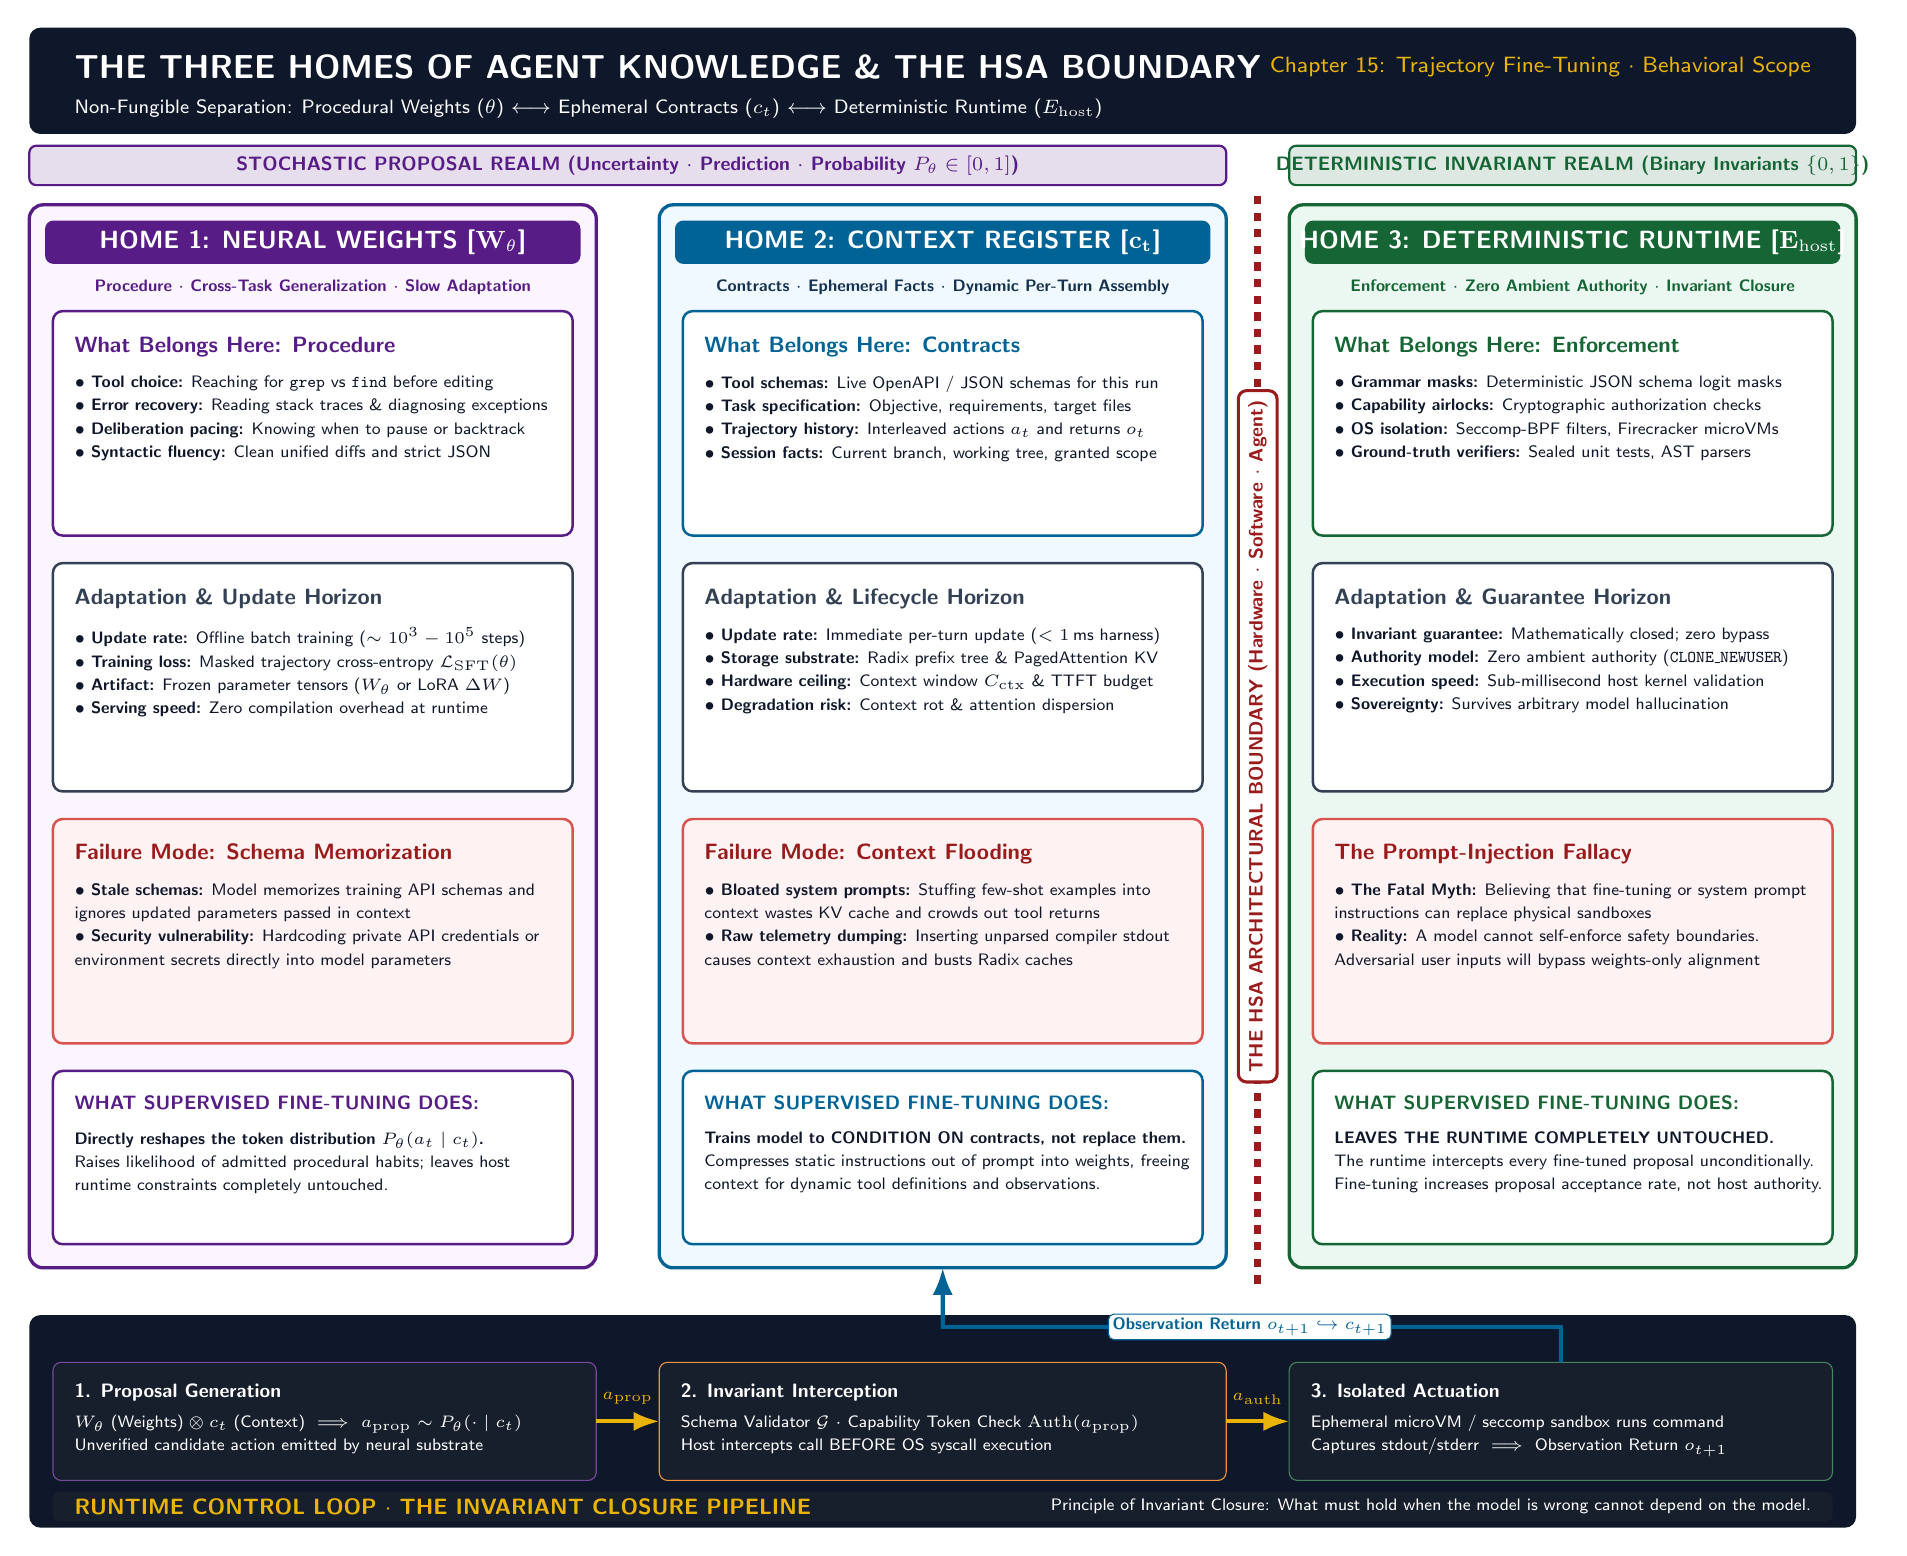
\begin{tikzpicture}[x=1cm, y=1cm]

% =============================================================================
% TOP TITLE BANNER (y: 18.2 to 19.55)
% =============================================================================
\draw[fill=DarkSlate, draw=none, rounded corners=4pt] (0, 18.2) rectangle (23.2, 19.55);
\node[anchor=west, font=\bfseries\large, text=white] at (0.45, 19.05) {
  THE THREE HOMES OF AGENT KNOWLEDGE \& THE HSA BOUNDARY
};
\node[anchor=east, font=\footnotesize, text=GoldPin] at (22.75, 19.05) {
  Chapter 15: Trajectory Fine-Tuning $\cdot$ Behavioral Scope
};
\node[anchor=west, font=\scriptsize, text=white!85] at (0.45, 18.52) {
  Non-Fungible Separation: Procedural Weights ($\theta$) $\longleftrightarrow$ Ephemeral Contracts ($c_t$) $\longleftrightarrow$ Deterministic Runtime ($E_{\mathrm{host}}$)
};

% Realm Indicator Strip (y: 17.55 to 18.05)
\draw[fill=amethyst!15, draw=amethyst, line width=0.8pt, rounded corners=2.5pt] (0, 17.55) rectangle (15.2, 18.05);
\node[font=\bfseries\fontsize{7pt}{8.5pt}\selectfont, text=amethyst] at (7.6, 17.8) {
  STOCHASTIC PROPOSAL REALM (Uncertainty $\cdot$ Prediction $\cdot$ Probability $P_\theta \in [0, 1]$)
};

\draw[fill=forestsage!15, draw=forestsage, line width=0.8pt, rounded corners=2.5pt] (16.0, 17.55) rectangle (23.2, 18.05);
\node[font=\bfseries\fontsize{7pt}{8.5pt}\selectfont, text=forestsage] at (19.6, 17.8) {
  DETERMINISTIC INVARIANT REALM (Binary Invariants $\{0, 1\}$)
};

% =============================================================================
% 1. LEFT CONTAINER: HOME 1 - NEURAL PARAMETER WEIGHTS (PROCEDURE)
% (x: 0 to 7.2, y: 3.8 to 17.3) - Height 13.5 cm
% =============================================================================
\draw[draw=amethyst, fill=amethystL0, line width=1.2pt, rounded corners=5pt] (0, 3.8) rectangle (7.2, 17.3);

% Header Bar
\fill[amethyst, rounded corners=3pt] (0.2, 16.55) rectangle (7.0, 17.1);
\node[font=\bfseries\small, text=white] at (3.6, 16.82) {
  HOME 1: NEURAL WEIGHTS [$\mathbf{W_\theta}$]
};
\node[font=\bfseries\fontsize{6.5pt}{7.5pt}\selectfont, text=amethyst] at (3.6, 16.25) {
  \textbf{Procedure} $\cdot$ Cross-Task Generalization $\cdot$ Slow Adaptation
};

% Block 1.1: What Belongs in Weights (y: 13.1 to 15.95) - height 2.85cm
\draw[draw=amethyst, fill=white, line width=0.9pt, rounded corners=3.5pt] (0.3, 13.1) rectangle (6.9, 15.95);
\node[anchor=north west, font=\bfseries\footnotesize, text=amethyst] at (0.45, 15.75) {What Belongs Here: Procedure};
\node[anchor=north west, font=\fontsize{6.5pt}{8.4pt}\selectfont, text=DarkSlate] at (0.45, 15.25) {
  \begin{minipage}{6.2cm}\raggedright
    $\bullet$ \textbf{Tool choice:} Reaching for \texttt{grep} vs \texttt{find} before editing\\
    $\bullet$ \textbf{Error recovery:} Reading stack traces \& diagnosing exceptions\\
    $\bullet$ \textbf{Deliberation pacing:} Knowing when to pause or backtrack\\
    $\bullet$ \textbf{Syntactic fluency:} Clean unified diffs and strict JSON
  \end{minipage}
};

% Block 1.2: Adaptation Mechanism (y: 9.85 to 12.75) - height 2.9cm
\draw[draw=slatesteel, fill=white, line width=0.9pt, rounded corners=3.5pt] (0.3, 9.85) rectangle (6.9, 12.75);
\node[anchor=north west, font=\bfseries\footnotesize, text=slatesteel] at (0.45, 12.55) {Adaptation \& Update Horizon};
\node[anchor=north west, font=\fontsize{6.5pt}{8.4pt}\selectfont, text=DarkSlate] at (0.45, 12.05) {
  \begin{minipage}{6.2cm}\raggedright
    $\bullet$ \textbf{Update rate:} Offline batch training ($\sim 10^3-10^5$ steps)\\
    $\bullet$ \textbf{Training loss:} Masked trajectory cross-entropy $\mathcal{L}_{\mathrm{SFT}}(\theta)$\\
    $\bullet$ \textbf{Artifact:} Frozen parameter tensors ($W_\theta$ or LoRA $\Delta W$)\\
    $\bullet$ \textbf{Serving speed:} Zero compilation overhead at runtime
  \end{minipage}
};

% Block 1.3: Anti-Pattern / Failure Mode (y: 6.65 to 9.5) - height 2.85cm
\draw[draw=RedLine, fill=RedL0, line width=0.9pt, rounded corners=3.5pt] (0.3, 6.65) rectangle (6.9, 9.5);
\node[anchor=north west, font=\bfseries\footnotesize, text=deepburgundy] at (0.45, 9.3) {Failure Mode: Schema Memorization};
\node[anchor=north west, font=\fontsize{6.5pt}{8.4pt}\selectfont, text=DarkSlate] at (0.45, 8.8) {
  \begin{minipage}{6.2cm}\raggedright
    $\bullet$ \textbf{Stale schemas:} Model memorizes training API schemas and ignores updated parameters passed in context\\
    $\bullet$ \textbf{Security vulnerability:} Hardcoding private API credentials or environment secrets directly into model parameters
  \end{minipage}
};

% Block 1.4: Fine-Tuning Impact Summary (y: 4.1 to 6.3) - height 2.2cm
\draw[draw=amethyst, fill=white, line width=0.9pt, rounded corners=3.5pt] (0.3, 4.1) rectangle (6.9, 6.3);
\node[anchor=north west, font=\bfseries\scriptsize, text=amethyst] at (0.45, 6.1) {WHAT SUPERVISED FINE-TUNING DOES:};
\node[anchor=north west, font=\fontsize{6.5pt}{8.4pt}\selectfont, text=DarkSlate] at (0.45, 5.65) {
  \begin{minipage}{6.2cm}\raggedright
    \textbf{Directly reshapes the token distribution $P_\theta(a_t \mid c_t)$.}\\
    Raises likelihood of admitted procedural habits; leaves host runtime constraints completely untouched.
  \end{minipage}
};

% =============================================================================
% 2. MIDDLE CONTAINER: HOME 2 - CONTEXT REGISTER (CONTRACTS)
% (x: 8.0 to 15.2, y: 3.8 to 17.3) - Height 13.5 cm
% =============================================================================
\draw[draw=BlueLine, fill=BlueL0, line width=1.2pt, rounded corners=5pt] (8.0, 3.8) rectangle (15.2, 17.3);

% Header Bar
\fill[BlueLine, rounded corners=3pt] (8.2, 16.55) rectangle (15.0, 17.1);
\node[font=\bfseries\small, text=white] at (11.6, 16.82) {
  HOME 2: CONTEXT REGISTER [$\mathbf{c_t}$]
};
\node[font=\bfseries\fontsize{6.5pt}{7.5pt}\selectfont, text=BlueDD] at (11.6, 16.25) {
  \textbf{Contracts} $\cdot$ Ephemeral Facts $\cdot$ Dynamic Per-Turn Assembly
};

% Block 2.1: What Belongs in Context (y: 13.1 to 15.95) - height 2.85cm
\draw[draw=BlueLine, fill=white, line width=0.9pt, rounded corners=3.5pt] (8.3, 13.1) rectangle (14.9, 15.95);
\node[anchor=north west, font=\bfseries\footnotesize, text=BlueLine] at (8.45, 15.75) {What Belongs Here: Contracts};
\node[anchor=north west, font=\fontsize{6.5pt}{8.4pt}\selectfont, text=DarkSlate] at (8.45, 15.25) {
  \begin{minipage}{6.2cm}\raggedright
    $\bullet$ \textbf{Tool schemas:} Live OpenAPI / JSON schemas for this run\\
    $\bullet$ \textbf{Task specification:} Objective, requirements, target files\\
    $\bullet$ \textbf{Trajectory history:} Interleaved actions $a_t$ and returns $o_t$\\
    $\bullet$ \textbf{Session facts:} Current branch, working tree, granted scope
  \end{minipage}
};

% Block 2.2: Adaptation Mechanism (y: 9.85 to 12.75) - height 2.9cm
\draw[draw=slatesteel, fill=white, line width=0.9pt, rounded corners=3.5pt] (8.3, 9.85) rectangle (14.9, 12.75);
\node[anchor=north west, font=\bfseries\footnotesize, text=slatesteel] at (8.45, 12.55) {Adaptation \& Lifecycle Horizon};
\node[anchor=north west, font=\fontsize{6.5pt}{8.4pt}\selectfont, text=DarkSlate] at (8.45, 12.05) {
  \begin{minipage}{6.2cm}\raggedright
    $\bullet$ \textbf{Update rate:} Immediate per-turn update ($< 1\,\text{ms}$ harness)\\
    $\bullet$ \textbf{Storage substrate:} Radix prefix tree \& PagedAttention KV\\
    $\bullet$ \textbf{Hardware ceiling:} Context window $C_{\mathrm{ctx}}$ \& TTFT budget\\
    $\bullet$ \textbf{Degradation risk:} Context rot \& attention dispersion
  \end{minipage}
};

% Block 2.3: Anti-Pattern / Failure Mode (y: 6.65 to 9.5) - height 2.85cm
\draw[draw=RedLine, fill=RedL0, line width=0.9pt, rounded corners=3.5pt] (8.3, 6.65) rectangle (14.9, 9.5);
\node[anchor=north west, font=\bfseries\footnotesize, text=deepburgundy] at (8.45, 9.3) {Failure Mode: Context Flooding};
\node[anchor=north west, font=\fontsize{6.5pt}{8.4pt}\selectfont, text=DarkSlate] at (8.45, 8.8) {
  \begin{minipage}{6.2cm}\raggedright
    $\bullet$ \textbf{Bloated system prompts:} Stuffing few-shot examples into context wastes KV cache and crowds out tool returns\\
    $\bullet$ \textbf{Raw telemetry dumping:} Inserting unparsed compiler stdout causes context exhaustion and busts Radix caches
  \end{minipage}
};

% Block 2.4: Fine-Tuning Impact Summary (y: 4.1 to 6.3) - height 2.2cm
\draw[draw=BlueLine, fill=white, line width=0.9pt, rounded corners=3.5pt] (8.3, 4.1) rectangle (14.9, 6.3);
\node[anchor=north west, font=\bfseries\scriptsize, text=BlueLine] at (8.45, 6.1) {WHAT SUPERVISED FINE-TUNING DOES:};
\node[anchor=north west, font=\fontsize{6.5pt}{8.4pt}\selectfont, text=DarkSlate] at (8.45, 5.65) {
  \begin{minipage}{6.2cm}\raggedright
    \textbf{Trains model to CONDITION ON contracts, not replace them.}\\
    Compresses static instructions out of prompt into weights, freeing context for dynamic tool definitions and observations.
  \end{minipage}
};

% =============================================================================
% 3. RIGHT CONTAINER: HOME 3 - DETERMINISTIC RUNTIME (ENFORCEMENT)
% (x: 16.0 to 23.2, y: 3.8 to 17.3) - Height 13.5 cm
% =============================================================================
\draw[draw=forestsage, fill=GreenL0, line width=1.2pt, rounded corners=5pt] (16.0, 3.8) rectangle (23.2, 17.3);

% Header Bar
\fill[forestsage, rounded corners=3pt] (16.2, 16.55) rectangle (23.0, 17.1);
\node[font=\bfseries\small, text=white] at (19.6, 16.82) {
  HOME 3: DETERMINISTIC RUNTIME [$\mathbf{E_{\mathrm{host}}}$]
};
\node[font=\bfseries\fontsize{6.5pt}{7.5pt}\selectfont, text=forestsage] at (19.6, 16.25) {
  \textbf{Enforcement} $\cdot$ Zero Ambient Authority $\cdot$ Invariant Closure
};

% Block 3.1: What Belongs in Runtime (y: 13.1 to 15.95) - height 2.85cm
\draw[draw=forestsage, fill=white, line width=0.9pt, rounded corners=3.5pt] (16.3, 13.1) rectangle (22.9, 15.95);
\node[anchor=north west, font=\bfseries\footnotesize, text=forestsage] at (16.45, 15.75) {What Belongs Here: Enforcement};
\node[anchor=north west, font=\fontsize{6.5pt}{8.4pt}\selectfont, text=DarkSlate] at (16.45, 15.25) {
  \begin{minipage}{6.2cm}\raggedright
    $\bullet$ \textbf{Grammar masks:} Deterministic JSON schema logit masks\\
    $\bullet$ \textbf{Capability airlocks:} Cryptographic authorization checks\\
    $\bullet$ \textbf{OS isolation:} Seccomp-BPF filters, Firecracker microVMs\\
    $\bullet$ \textbf{Ground-truth verifiers:} Sealed unit tests, AST parsers
  \end{minipage}
};

% Block 3.2: Adaptation Mechanism (y: 9.85 to 12.75) - height 2.9cm
\draw[draw=slatesteel, fill=white, line width=0.9pt, rounded corners=3.5pt] (16.3, 9.85) rectangle (22.9, 12.75);
\node[anchor=north west, font=\bfseries\footnotesize, text=slatesteel] at (16.45, 12.55) {Adaptation \& Guarantee Horizon};
\node[anchor=north west, font=\fontsize{6.5pt}{8.4pt}\selectfont, text=DarkSlate] at (16.45, 12.05) {
  \begin{minipage}{6.2cm}\raggedright
    $\bullet$ \textbf{Invariant guarantee:} Mathematically closed; zero bypass\\
    $\bullet$ \textbf{Authority model:} Zero ambient authority (\texttt{CLONE\_NEWUSER})\\
    $\bullet$ \textbf{Execution speed:} Sub-millisecond host kernel validation\\
    $\bullet$ \textbf{Sovereignty:} Survives arbitrary model hallucination
  \end{minipage}
};

% Block 3.3: Anti-Pattern / Failure Mode (y: 6.65 to 9.5) - height 2.85cm
\draw[draw=RedLine, fill=RedL0, line width=0.9pt, rounded corners=3.5pt] (16.3, 6.65) rectangle (22.9, 9.5);
\node[anchor=north west, font=\bfseries\footnotesize, text=deepburgundy] at (16.45, 9.3) {The Prompt-Injection Fallacy};
\node[anchor=north west, font=\fontsize{6.5pt}{8.4pt}\selectfont, text=DarkSlate] at (16.45, 8.8) {
  \begin{minipage}{6.2cm}\raggedright
    $\bullet$ \textbf{The Fatal Myth:} Believing that fine-tuning or system prompt instructions can replace physical sandboxes\\
    $\bullet$ \textbf{Reality:} A model cannot self-enforce safety boundaries. Adversarial user inputs will bypass weights-only alignment
  \end{minipage}
};

% Block 3.4: Fine-Tuning Impact Summary (y: 4.1 to 6.3) - height 2.2cm
\draw[draw=forestsage, fill=white, line width=0.9pt, rounded corners=3.5pt] (16.3, 4.1) rectangle (22.9, 6.3);
\node[anchor=north west, font=\bfseries\scriptsize, text=forestsage] at (16.45, 6.1) {WHAT SUPERVISED FINE-TUNING DOES:};
\node[anchor=north west, font=\fontsize{6.5pt}{8.4pt}\selectfont, text=DarkSlate] at (16.45, 5.65) {
  \begin{minipage}{6.2cm}\raggedright
    \textbf{LEAVES THE RUNTIME COMPLETELY UNTOUCHED.}\\
    The runtime intercepts every fine-tuned proposal unconditionally. Fine-tuning increases proposal acceptance rate, not host authority.
  \end{minipage}
};

% =============================================================================
% 4. HSA ARCHITECTURAL BOUNDARY (THE DEMARCATION LINE)
% =============================================================================
\draw[draw=deepburgundy, line width=2.4pt, dashed] (15.6, 3.6) -- (15.6, 17.5);
\node[draw=deepburgundy, fill=white, line width=1.1pt, rounded corners=3pt, inner sep=3.5pt, font=\bfseries\scriptsize, text=deepburgundy, rotate=90] 
  at (15.6, 10.55) {THE HSA ARCHITECTURAL BOUNDARY (Hardware $\cdot$ Software $\cdot$ Agent)};

% =============================================================================
% 5. BOTTOM TIER: INTER-HOME RUNTIME DATAPATH
% (x: 0 to 23.2, y: 0.5 to 3.2)
% =============================================================================
\draw[fill=DarkSlate, draw=none, rounded corners=4pt] (0, 0.5) rectangle (23.2, 3.2);

% Sub-blocks in Bottom Bus
% Bus 1: Model Proposal Generation (Home 1 + Home 2)
\draw[draw=amethyst!80, fill=ChipBlack, rounded corners=3pt] (0.3, 1.1) rectangle (7.2, 2.6);
\node[anchor=north west, font=\bfseries\scriptsize, text=white] at (0.45, 2.45) {1. Proposal Generation};
\node[anchor=north west, font=\fontsize{6.5pt}{8.2pt}\selectfont, text=white!80] at (0.45, 2.05) {
  \begin{minipage}{6.5cm}\raggedright
    $W_\theta \text{ (Weights)} \otimes c_t \text{ (Context)} \implies a_{\mathrm{prop}} \sim P_\theta(\cdot \mid c_t)$\\
    Unverified candidate action emitted by neural substrate
  \end{minipage}
};

% Bus 2: Capability Interceptor & Airlock (Home 3 Entry)
\draw[draw=OrangeLine!80, fill=ChipBlack, rounded corners=3pt] (8.0, 1.1) rectangle (15.2, 2.6);
\node[anchor=north west, font=\bfseries\scriptsize, text=white] at (8.15, 2.45) {2. Invariant Interception};
\node[anchor=north west, font=\fontsize{6.5pt}{8.2pt}\selectfont, text=white!80] at (8.15, 2.05) {
  \begin{minipage}{6.8cm}\raggedright
    Schema Validator $\mathcal{G}$ $\cdot$ Capability Token Check $\mathrm{Auth}(a_{\mathrm{prop}})$\\
    Host intercepts call BEFORE OS syscall execution
  \end{minipage}
};

% Bus 3: Hermetic Sandboxed Execution
\draw[draw=forestsage!80, fill=ChipBlack, rounded corners=3pt] (16.0, 1.1) rectangle (22.9, 2.6);
\node[anchor=north west, font=\bfseries\scriptsize, text=white] at (16.15, 2.45) {3. Isolated Actuation};
\node[anchor=north west, font=\fontsize{6.5pt}{8.2pt}\selectfont, text=white!80] at (16.15, 2.05) {
  \begin{minipage}{6.4cm}\raggedright
    Ephemeral microVM / seccomp sandbox runs command\\
    Captures stdout/stderr $\implies$ Observation Return $o_{t+1}$
  \end{minipage}
};

% Bus arrows
\draw[flow_arrow, draw=GoldPin, line width=1.4pt] (7.2, 1.85) -- node[above=2pt, font=\bfseries\fontsize{6pt}{7pt}\selectfont, text=GoldPin] {$a_{\mathrm{prop}}$} (8.0, 1.85);
\draw[flow_arrow, draw=GoldPin, line width=1.4pt] (15.2, 1.85) -- node[above=2pt, font=\bfseries\fontsize{6pt}{7pt}\selectfont, text=GoldPin] {$a_{\mathrm{auth}}$} (16.0, 1.85);

% Observation Return Loop back to Context (Home 2)
\draw[flow_arrow, draw=BlueLine, line width=1.5pt] 
  (19.45, 2.6) -- ++(0, 0.45) -- ++(-7.85, 0) -- (11.6, 3.8);
\node[draw=BlueLine, fill=white, rounded corners=2pt, inner sep=1.5pt, font=\bfseries\fontsize{6pt}{7pt}\selectfont, text=BlueLine] 
  at (15.5, 3.05) {Observation Return $o_{t+1} \hookrightarrow c_{t+1}$};

% Title Strip inside bus at the BOTTOM
\fill[ChipBlack, rounded corners=2pt] (0.3, 0.58) rectangle (22.9, 0.95);
\node[anchor=west, font=\bfseries\footnotesize, text=GoldPin] at (0.45, 0.77) {
  RUNTIME CONTROL LOOP $\cdot$ THE INVARIANT CLOSURE PIPELINE
};
\node[anchor=east, font=\fontsize{6.5pt}{8pt}\selectfont, text=white!80] at (22.75, 0.77) {
  Principle of Invariant Closure: What must hold when the model is wrong cannot depend on the model.
};

\end{tikzpicture}
\end{document}
